\documentclass[11pt]{article}

\usepackage[margin=1in]{geometry}
\usepackage[utf8]{inputenc}
\usepackage[T1]{fontenc}
\usepackage{charter}
\usepackage{amsmath,amssymb}
\usepackage{booktabs}
\usepackage[numbers]{natbib}
\usepackage{float}
\usepackage{xurl}
\usepackage{hyperref}
\usepackage{enumitem}
\usepackage{caption}
\usepackage{titlesec}
\usepackage{xcolor}
\usepackage{graphicx}
\usepackage{tikz}
\usetikzlibrary{positioning,arrows.meta,fit}

\hypersetup{colorlinks=true,linkcolor=black,citecolor=black,urlcolor=blue!50!black}
\titleformat{\section}{\normalfont\large\bfseries}{\thesection}{0.6em}{}
\titleformat{\subsection}{\normalfont\bfseries}{\thesubsection}{0.6em}{}
\captionsetup{font=small,skip=4pt}
\setlength{\textfloatsep}{10pt plus 2pt minus 2pt}

\title{\textbf{Fostering Epistemic Diversity in the AI Era}}

\author{
Sofia G. Gallego$^{1}$ \\[4pt]
\normalsize $^1$CosmoVentures, Paris, France, with Apart Research
}
\date{Apart Research AI $\times$ Epistemics Research Sprint, November 2026}

\begin{document}
\maketitle

\begin{abstract}
Creativity, innovation and improvement often happen in the space between ideas. As more of our thinking passes through AI, that space can quietly shrink, or it can grow. Evidence from science, art, politics, law, culture and work points the same way: each person gains, and the whole loses range. This position paper outlines directions in which the community can foster epistemic diversity, and proposes one concrete step: a public map of ideas, where concepts are seen from many perspectives and the space between them stays in view, tested against the range of ideas real people reach.
\end{abstract}

\section{Introduction}

A word like \emph{water} reads differently to a chemist, a farmer, a historian and a poet. Each reading is true, and new ideas often appear where two of them meet. Groups that think in different ways find what groups of the individually best problem solvers miss \citep{hong2004}, and the most cited science tends to join familiar ideas in unusual combinations \citep{uzzi2013}. The world is more connected than ever, and so are its questions: climate, health, technology and justice cross every border between fields.

How can people and AI think together in a way that keeps the space between ideas open, and even widens it? A harmonic interaction would keep what works in each and enhance what can be enhanced. Section~2 gathers what is at stake across fields, Section~3 what has been tried, Section~4 where the community could go, and Section~5 proposes a map of ideas.

\section{Background}

Across many fields the same pattern appears: each person gains, and the whole loses range.

\textbf{Science and creativity.} Researchers who use AI publish more and are cited more, while the range of topics studied together shrinks \citep{hao2026}, and questions that suit AI can crowd out others \citep{messeri2024}. Writers and artists helped by AI produce work judged better, which becomes more alike over time \citep{doshi2024,zhou2024,anderson2024}.

\textbf{Politics, law and institutions.} People who write with a model that leans toward one view move their own opinions toward it \citep{jakesch2023}. When many decision makers use the same model, their errors stop being independent, and the same people are wrongly rejected everywhere \citep{kleinberg2021,bommasani2022}.

\textbf{Culture and representation.} Models answer most like people in Western, rich societies \citep{atari2023,durmus2024}, image generators amplify stereotypes \citep{bianchi2023}, most languages have almost no place in language technology \citep{joshi2020}, and writing suggestions pull other cultures toward Western styles \citep{agarwal2025}. Bias and homogenization are one problem seen from two sides: whose perspective becomes the default.

\textbf{Work, learning and power.} The first jobs to thin out are those where young people start a career \citep{eloundou2024,brynjolfsson2025}, and fewer people entering a field means fewer perspectives growing inside it. Students who write with AI write more alike and remember less \citep{kosmyna2025}. A few providers build the models most people think with \citep{korinek2025}, and whether they replace people or extend them is a choice \citep{acemoglu2023}.

\textbf{The models.} Chat training reduces variety \citep{kirk2024}, models are more alike than people \citep{wenger2026,jiang2025}, and rare ideas can fade from use, a process called knowledge collapse \citep{peterson2024,wright2025}.

\section{Related Work}

\textbf{Measuring diversity.} Benchmarks ask whether models give humanlike variety \citep{zhang2025} and how much of the world's knowledge they cover \citep{wright2025}.

\textbf{Widening models.} Personas and backstories make the answers of models more varied \citep{moon2024,deng2026}.

\textbf{Tools for groups.} Polis maps opinions so groups see where they differ \citep{polis2021}, Community Notes shows a note only when people who usually disagree both find it helpful \citep{wojcik2022}, and the Habermas Machine drafts statements a divided group can share \citep{tessler2024}. Each works on a question already asked. The space between ideas, where new questions come from, has fewer tools.

\textbf{Earlier work by the author.} Two earlier studies led to this proposal. In False epistemic redundancy, with a collaborator, AI agents given different reasoning personas sounded different and still missed the same cause \citep{gallego2026fer}. In Epistemic Bridges, made during this sprint, people and models link the same pairs of words, and each model is placed on the map that people's answers draw \citep{gallego2026bridges}: the newer chat models reached less of it than people, even with their shared voice removed, and answering as an ordinary person drawn at random was the one change that widened every model's ideas. Steering a small model's activations toward that perspective brought it to the range of people while its knowledge and safety held.

\section{Directions}

The community can foster epistemic diversity by measuring it against what real people do, alongside accuracy and safety; by giving models perspectives and lives alongside better reasoning, and keeping several independent models in use where decisions affect many people; by building tools that show what lies around an idea before an answer settles it; by bringing fields and cultures together in debates and interdisciplinary residencies; by protecting the languages, cultures and entry-level work the market leaves out; and by carrying the evidence into policy and schools.

\section{Proposal: The Map of Ideas}

The step proposed here is a non-linear Wikipedia: a shared space where knowledge is read through its connections.

The idea has a long history. Vannevar Bush imagined a machine that would keep the associative trails a reader makes between documents \citep{bush1945}, and Ted Nelson proposed links that run both ways \citep{nelson1965}. Concept maps draw ideas and the relations between them for teaching \citep{novak2008}, Wikidata links facts into one open graph \citep{vrandecic2014}, and Kialo (\href{https://www.kialo.com}{kialo.com}) arranges the arguments for and against a single claim as a tree. Wikipedia itself is read one article at a time.

The Map of Ideas (\href{https://mapideas.org}{mapideas.org}, Figure~\ref{fig:map}) brings these threads together around the space between ideas. A link carries how one idea reads from the other, in both directions. A criticism or answer is an idea of its own, joined to what it answers, so different views stand side by side and nothing is ranked. Ideas connect across fields, from mathematics and astronomy to religions, cultures and art, and any idea can become the center. Each tradition is described as its own people would. An AI guide answers from the map and never writes to it. A first version holds more than 300 ideas and open questions across 17 topics.

\begin{figure}[H]
\centering
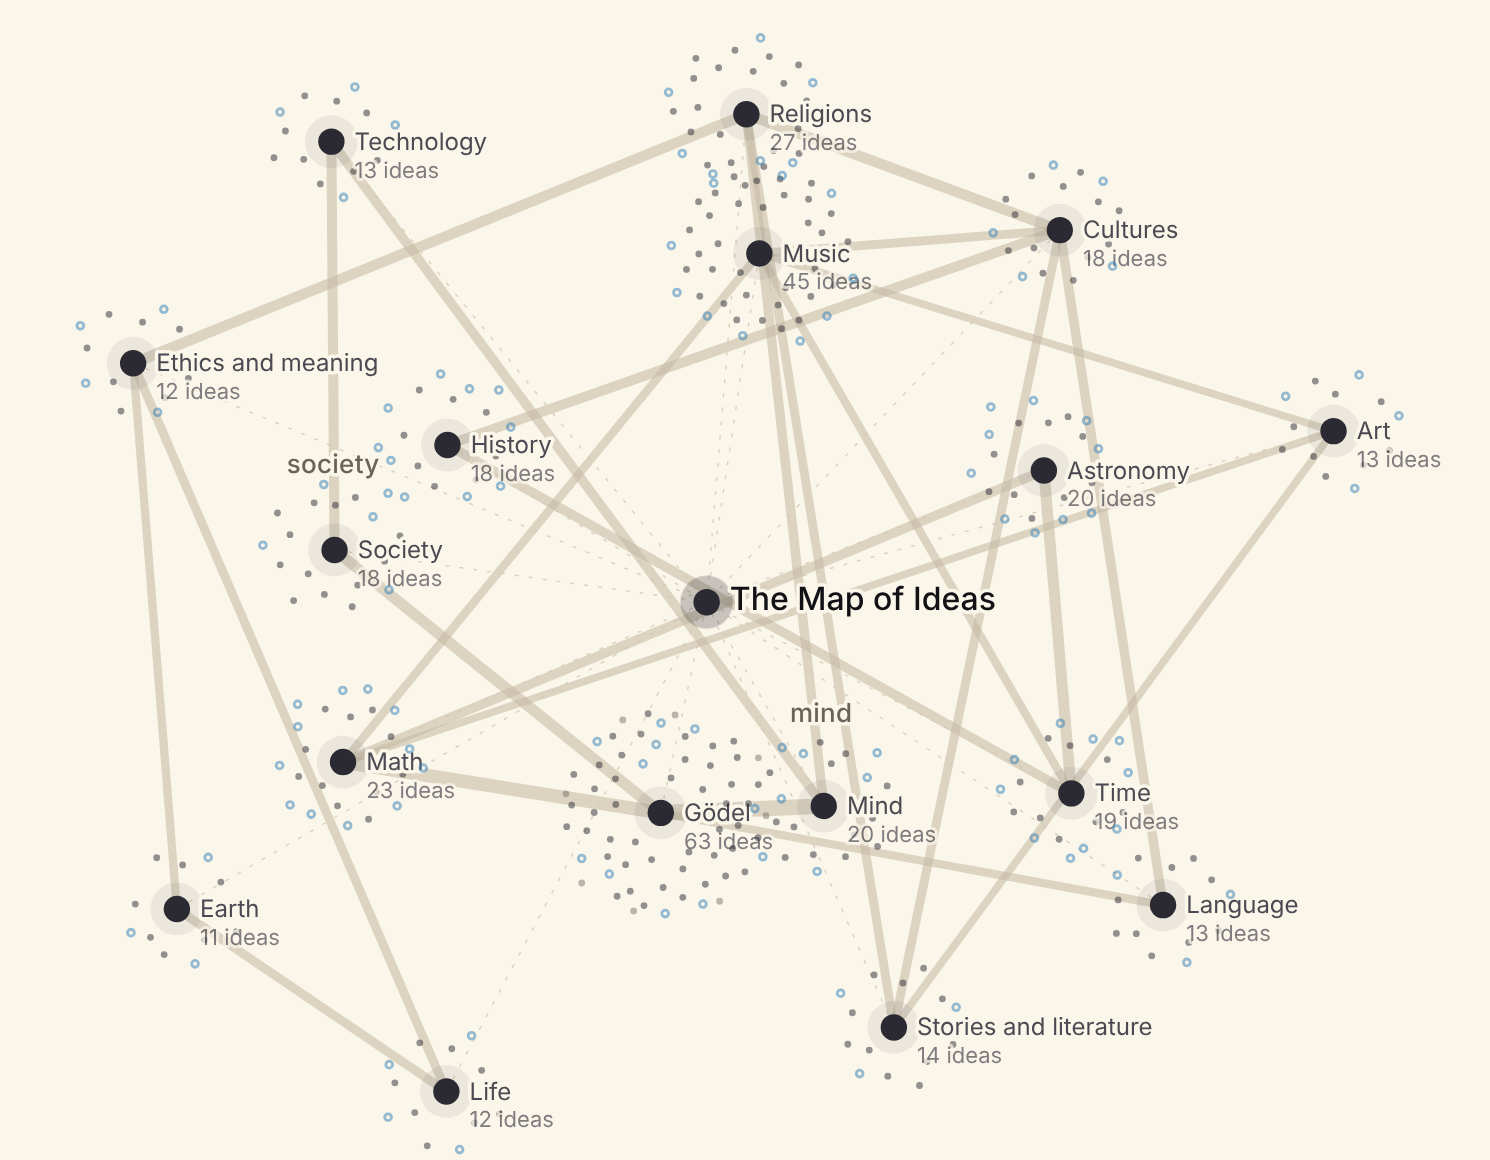
\includegraphics[width=0.60\textwidth]{map_overview.png}\hfill
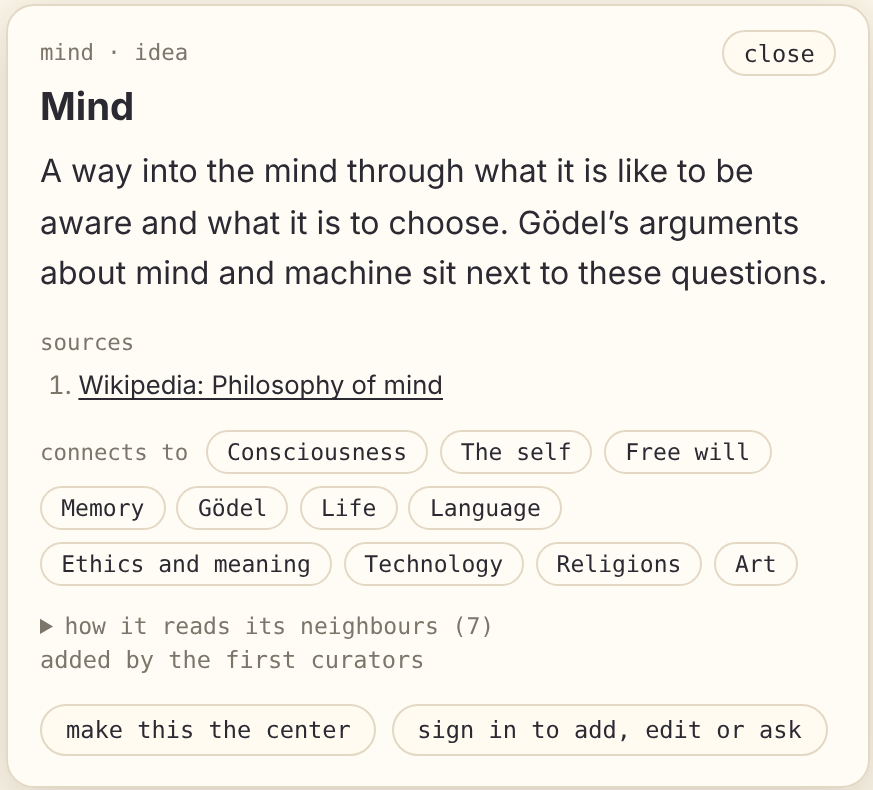
\includegraphics[width=0.37\textwidth]{map_card.png}
\caption{The Map of Ideas. Left, the whole map: topics and the lines between them, thicker where more ideas connect, with each topic's ideas around it. Right, an idea as a reader sees it, with its sources, the ideas it connects to across topics, and how it reads each neighbour.}
\label{fig:map}
\end{figure}

\textbf{For people outside a field.} A map can also be read by someone who is not an expert. A reader sees the positions around a question and how they relate, and can follow a thread from what they know into what they do not. They can also add their own view, with its own biases and visions, next to the others, where it can be read and answered. For outreach, teaching and public debate, this turns a field into a place to walk through, and opens it to people who would not enter it through its papers.

\textbf{How it could grow.} Topics written with the people of each field, tradition and language, so that no single view becomes the center. Personal maps grown from people's own notes, shared by choice. Trails through ideas, saved and passed on. Debates and interdisciplinary residencies held on the map, so that what they find stays for others.

\textbf{How to know it works.} A map shown to everyone is also a shared prior: it could widen what people reach, or become the new common answer. Bridges gives a way to tell. Players link the same words alone, after exploring the map, or after seeing a bridge from an AI, and each group is read against a reference map drawn by other players. The map fosters diversity if the group that used it reaches further and still lands where people go. After answering, players could also see where their own connection sits among everyone's.

\section{Conclusion}

The choices that shape how AI meets the space of ideas rest today with few, and the directions that could widen it belong to many. A map of ideas, tested against the range real people reach, is one place to start: if it widens what people find, it can grow with them; if it narrows it, the test will show that too.

This proposal is itself shaped by one perspective. The map was started by one person, is written mostly in English, and its first topics follow her interests. That is one more reason to test it against people other than its author, and to open it to the people of each field and tradition, so that the map grows beyond the view it started from.

\section*{Data and Code Availability}
The Map of Ideas is at \url{https://mapideas.org}, and the Bridges game at \url{https://mapideas.org/bridges}; their code, and this paper in the \texttt{paper/} folder, are at \url{https://github.com/nefinia/mapideas}. The Bridges measures, AI answers and analysis are at \url{https://github.com/nefinia/epistemic-bridges}, and the steering pilot at \url{https://github.com/nefinia/steering-the-voice}. The Map of Ideas, the game and false epistemic redundancy existed before the sprint started on 13 November; the Bridges study, the steering pilot and this paper were made during it.

\section*{Author Contributions and Acknowledgements}
S.G.G.\ conceived the vision, the map, the game and the studies, and wrote this paper with Claude (see LLM Usage Statement). Thanks to everyone who played Bridges and left feedback.

\begin{thebibliography}{99}
\small
\bibitem{hong2004} L.\ Hong, S.\ E.\ Page. \emph{Groups of diverse problem solvers can outperform groups of high-ability problem solvers.} PNAS, 101(46), 2004.
\bibitem{uzzi2013} B.\ Uzzi, S.\ Mukherjee, M.\ Stringer, B.\ Jones. \emph{Atypical combinations and scientific impact.} Science, 342(6157), 2013.
\bibitem{hao2026} Q.\ Hao, F.\ Xu, Y.\ Li, J.\ Evans. \emph{AI Expands Scientists' Impact but Contracts Science's Focus.} Nature (accepted), 2026. arXiv:2412.07727.
\bibitem{messeri2024} L.\ Messeri, M.\ J.\ Crockett. \emph{Artificial intelligence and illusions of understanding in scientific research.} Nature, 627, 2024.
\bibitem{doshi2024} A.\ R.\ Doshi, O.\ P.\ Hauser. \emph{Generative AI enhances individual creativity but reduces the collective diversity of novel content.} Science Advances, 10(28), 2024.
\bibitem{zhou2024} E.\ Zhou, D.\ Lee. \emph{Generative artificial intelligence, human creativity, and art.} PNAS Nexus, 3(3), 2024.
\bibitem{anderson2024} B.\ R.\ Anderson, J.\ H.\ Shah, M.\ Kreminski. \emph{Homogenization Effects of Large Language Models on Human Creative Ideation.} Creativity \& Cognition, 2024.
\bibitem{jakesch2023} M.\ Jakesch, A.\ Bhat, D.\ Buschek, L.\ Zalmanson, M.\ Naaman. \emph{Co-Writing with Opinionated Language Models Affects Users' Views.} CHI, 2023.
\bibitem{tessler2024} M.\ H.\ Tessler et al. \emph{AI can help humans find common ground in democratic deliberation.} Science, 386(6719), 2024.
\bibitem{kleinberg2021} J.\ Kleinberg, M.\ Raghavan. \emph{Algorithmic monoculture and social welfare.} PNAS, 118(22), 2021.
\bibitem{bommasani2022} R.\ Bommasani, K.\ A.\ Creel, A.\ Kumar, D.\ Jurafsky, P.\ Liang. \emph{Picking on the Same Person: Does Algorithmic Monoculture lead to Outcome Homogenization?} NeurIPS, 2022.
\bibitem{agarwal2025} D.\ Agarwal, M.\ Naaman, A.\ Vashistha. \emph{AI Suggestions Homogenize Writing Toward Western Styles and Diminish Cultural Nuances.} CHI, 2025.
\bibitem{kosmyna2025} N.\ Kosmyna et al. \emph{Your Brain on ChatGPT: Accumulation of Cognitive Debt when Using an AI Assistant for Essay Writing Task.} arXiv:2506.08872, 2025.
\bibitem{kirk2024} R.\ Kirk, I.\ Mediratta, C.\ Nalmpantis, J.\ Luketina, E.\ Hambro, E.\ Grefenstette, R.\ Raileanu. \emph{Understanding the Effects of RLHF on LLM Generalisation and Diversity.} ICLR, 2024.
\bibitem{wenger2026} E.\ Wenger, Y.\ N.\ Kenett. \emph{Large language models are homogeneously creative.} PNAS Nexus, 5(3):pgag042, 2026.
\bibitem{jiang2025} L.\ Jiang et al. \emph{Artificial Hivemind: The Open-Ended Homogeneity of Language Models (and Beyond).} NeurIPS, 2025.
\bibitem{peterson2024} A.\ J.\ Peterson. \emph{AI and the Problem of Knowledge Collapse.} arXiv:2404.03502, 2024.
\bibitem{wright2025} D.\ Wright, S.\ Masud, J.\ Moore, S.\ Yadav, M.\ Antoniak, P.\ Ebert Christensen, C.\ Y.\ Park, I.\ Augenstein. \emph{Epistemic Diversity and Knowledge Collapse in Large Language Models.} arXiv:2510.04226, 2025.
\bibitem{zhang2025} Y.\ Zhang, H.\ Diddee, S.\ Holm, H.\ Liu, X.\ Liu, V.\ Samuel, B.\ Wang, D.\ Ippolito. \emph{NoveltyBench: Evaluating Language Models for Humanlike Diversity.} arXiv:2504.05228, 2025.
\bibitem{moon2024} S.\ Moon et al. \emph{Virtual Personas for Language Models via an Anthology of Backstories.} EMNLP, 2024.
\bibitem{deng2026} Y.\ Deng, M.\ Brucks, O.\ Toubia. \emph{Examining and Addressing Barriers to Diversity in LLM-Generated Ideas.} 2026.
\bibitem{polis2021} C.\ Small, M.\ Bjorkegren, T.\ Erkkilä, L.\ Shaw, C.\ Megill. \emph{Polis: Scaling Deliberation by Mapping High Dimensional Opinion Spaces.} Recerca, 26(2), 2021.
\bibitem{wojcik2022} S.\ Wojcik et al. \emph{Birdwatch: Crowd Wisdom and Bridging Algorithms can Inform Understanding and Reduce the Spread of Misinformation.} arXiv:2210.15723, 2022.
\bibitem{gallego2026fer} S.\ G.\ Gallego, A.\ Habana. \emph{False Epistemic Redundancy: Do AI Ensembles Share a Blind Spot?} Apart Research Digital Minds Research Sprint, 2026. \url{https://apartresearch.com/project/false-epistemic-redundancy-do-ai-ensembles-share-a-blind-spot-b50u}
\bibitem{gallego2026bridges} S.\ G.\ Gallego. \emph{Epistemic Bridges: Do Language Models Reach the Connections People Make?} Apart Research AI $\times$ Epistemics Research Sprint, 2026. \url{https://apartresearch.com/sprints/projects/epistemic-bridges-do-language-models-reach-the-connections-people-make-y0xuxrgxw8}
\bibitem{eloundou2024} T.\ Eloundou, S.\ Manning, P.\ Mishkin, D.\ Rock. \emph{GPTs are GPTs: Labor market impact potential of LLMs.} Science, 384(6702), 2024.
\bibitem{brynjolfsson2025} E.\ Brynjolfsson, B.\ Chandar, R.\ Chen. \emph{Canaries in the Coal Mine? Six Facts about the Recent Employment Effects of Artificial Intelligence.} Stanford Digital Economy Lab, 2025.
\bibitem{acemoglu2023} D.\ Acemoglu, S.\ Johnson. \emph{Power and Progress: Our Thousand-Year Struggle Over Technology and Prosperity.} PublicAffairs, 2023.
\bibitem{korinek2025} A.\ Korinek, J.\ Vipra. \emph{Concentrating Intelligence: Scaling and Market Structure in Artificial Intelligence.} Economic Policy, 40(121), 2025.
\bibitem{atari2023} M.\ Atari, M.\ J.\ Xue, P.\ S.\ Park, D.\ E.\ Blasi, J.\ Henrich. \emph{Which Humans?} PsyArXiv, 2023.
\bibitem{durmus2024} E.\ Durmus et al. \emph{Towards Measuring the Representation of Subjective Global Opinions in Language Models.} COLM, 2024.
\bibitem{bianchi2023} F.\ Bianchi et al. \emph{Easily Accessible Text-to-Image Generation Amplifies Demographic Stereotypes at Large Scale.} FAccT, 2023.
\bibitem{joshi2020} P.\ Joshi, S.\ Santy, A.\ Budhiraja, K.\ Bali, M.\ Choudhury. \emph{The State and Fate of Linguistic Diversity and Inclusion in the NLP World.} ACL, 2020.
\bibitem{bush1945} V.\ Bush. \emph{As We May Think.} The Atlantic Monthly, July 1945.
\bibitem{nelson1965} T.\ H.\ Nelson. \emph{Complex information processing: a file structure for the complex, the changing and the indeterminate.} ACM National Conference, 1965.
\bibitem{novak2008} J.\ D.\ Novak, A.\ J.\ Cañas. \emph{The Theory Underlying Concept Maps and How to Construct and Use Them.} Technical Report IHMC CmapTools 2006-01 Rev 01-2008, Florida Institute for Human and Machine Cognition, 2008.
\bibitem{vrandecic2014} D.\ Vrandečić, M.\ Krötzsch. \emph{Wikidata: a free collaborative knowledgebase.} Communications of the ACM, 57(10), 2014.
\end{thebibliography}

\section*{LLM Usage Statement}
Claude helped build the Map of Ideas and the Bridges game before the sprint. During it, Claude searched for and checked the literature, drafted and revised this paper with the author, and made the figure of the map; the ideas, the framing and the proposal are the author's, and she directed every revision. All numbers come from the cited studies and from the analysis scripts of the Bridges study and the steering pilot.

\end{document}
